\documentclass[11pt]{article}
\usepackage[utf8]{inputenc}
\usepackage{longtable}
\usepackage{color}
\usepackage{multirow}
\usepackage{hyperref}
\usepackage{setspace}
%\doublespacing

\renewcommand*{\sectionautorefname}{Section} 

\title{Documentation\_SM \\ Policy emergence model}
\author{Raphael Klein}

\usepackage{natbib}
\usepackage{graphicx}
\usepackage[labelfont=bf]{caption} 	% Make captions bold (Figure & Table)
\usepackage{subfig}	
\usepackage{amsmath}
\usepackage{hyperref}
%\usepackage[section]{placeins}

\providecommand{\keywords}[1]{\textbf{Keywords:} #1}

\begin{document}

\maketitle

%\begin{center}
%Word count: 9300 words
%\end{center}


\tableofcontents

%%%%%%%%%%%%%%%%%%%%%%%%%%%%%%%%
\section{Model conceptualisation}

The policy process model is specified according to the four key elements that were outlined in the literature: time, policy arena, agents and interactions. The main choice that is left to the modeller is to decide how much complexity needs to be integrated to each of these elements to answer the research question. In the present case, only a limited amount of complexity is required. This leads to a relatively simple policymaking process model. It is detailed below.

%%%%%%%%%%%%%%%%
\subsection{Time}

For the time element, we consider a two step policymaking process consisting of an agenda setting and a policy formulation step. The agenda setting step is the first step, and consists of the agents selecting an issue to place on the agenda to narrow down further discussions. This agenda is then used to limit the policy instruments that can be evaluated for implementation. During the policy formulation step, the policy makers select a policy instrument and implement it with the aim of affecting the outcomes of the electricity model.

%%%%%%%%%%%%%%%% end of the time subsection

%%%%%%%%%%%%%%%%
\subsection{The policy arena}

This policy arena helps define the issues that can be considered within the belief system of the agents. It further limits the agents that can be considered to policy makers that are related to the environment model. It also helps define the policy instruments that can be considered within this model. No deep core issues are considered within this application as they are considered out of the scope of the model.

%%%%%%%%%%%%%%%% end of the policy arena subsection

%%%%%%%%%%%%%%%%
\subsection{The agents and the environment}

For the agents, only two roles are retained: the policy makers and the electorate. The policy makers are agents that decide what should go on the agenda and what policies should be implemented. They base their decisions on their preferred states and their beliefs for each issue in the belief tree. They focus on the issues that they consider to be the most urgent to deal with, which means issues that have the largest gap between preferred state and belief. The electorate on the other hand can only perform one action: they influence the preferred states of the policy makers. This influence is a progressive influence that can vary in speed based on a modeller defined parameter.

%%%%%%%%%%%%%%%% end of the actors and environment subsection

%%%%%%%%%%%%%%%%
\subsection{The interactions}

When it comes to the interactions, only three are considered. As outlined in the previous paragraph, the first interaction is the electorate influencing the policy makers. The second and third interactions are then inherent in the construction of the hybrid model: the environment - electricity market, influences the beliefs of the policy makers, and, through policy instruments, the policy makers influence the environment model.

%%%%%%%%%%%%%%%% end of the interactions subsection
%%%%%%%%%%%%%%%%%%%%%%%%%%%%%%%% end of the model conceptualisation section


%%%%%%%%%%%%%%%%%%%%%%%%%%%%%%%%
\section{Model formalisation}

%%%%%%%%%%%%%%%%
\subsection{The process}

In the simplest model, we assume that the policy process followed is a two-step process. First the agenda setting step is performed, then, if an agenda has bene agreed on, comes the policy formulation step. This does not include the environment simulation that is outlined in the next section.

The steps used to mode this approach are then detailed as follows:

\begin{enumerate}
\item Initialisation:
	
	\begin{enumerate}
	\item \emph{Trigger of external events:} Any event that the modeller decides to implement are activated at this stage of the model cycle.
	\item \emph{Update of the truth agent:} Information from the environment is used to inform the truth agent actual beliefs.
	\item \emph{Electorate actions on policy makers}
	\item \emph{Transmission of the actual beliefs:} The agents are informed about the environment from the truth agent.
	\end{enumerate}
	
\item Agenda setting step:
	\begin{enumerate}
	\item \emph{Preferences calculation (issues):} Each agent calculates the preference for their deep core and policy core issues. Additionally, each agents selects an issue that (s)he will advocate for in his/her policy core issues based on the preferences.
	\item \emph{Agenda selection}
	\end{enumerate}
	
\item Policy formulation step:
	\begin{enumerate}
	\item \emph{Preferences calculation (policy instruments):} All agents update their preferences for their secondary beliefs based on the issue on the agenda. All agents then selects a policy instrument that (s)he will be advocating for.
	\item \emph{Policy instrument implementation} 
	\end{enumerate}

\end{enumerate}

%%%%%%%%%%%%%%%% end of the process subsection

%%%%%%%%%%%%%%%%
\subsection{The agents}

There are two main categories of agents in the model: the active agents that have a direct influence on the agenda and the passive agents that an indirect impact on the agenda and policy change.

%%%%%%
\paragraph{Active agents}

The active agents are the policy makers. Their attributes are given as follows:

\begin{enumerate}

\item The \emph{active agent} is represented as an 4-tuple given by \texttt{agent = (ID, type, beliefHierarchy, advocacy)} where
\texttt{ID} is the agent unique ID,
\texttt{type} is the agent type, 
\texttt{beliefHierarchy} is the agent's personalised belief hierarchy, 
\texttt{advocacy} is the list of the issues the agent is supporting.

\item A \emph{type} corresponds the agent type: in this case it can only be a policy maker. This will go on to define the actions possible for the agent.

\item The \emph{belief hierarchy} is made of the agent's own belief hierarchy structure and associated values.

\item The \emph{advocacy} is represented as a 2-tuple \texttt{(issue\_as, issue\_pf)} where \texttt{policy\_pf} is the issue chosen by the agent during the agenda setting step, while the \texttt{policy\_pf} is the policy instrument selected by the agent in the policy formulation step.

\end{enumerate}

%%%%%% end of the active agents paragraph

%%%%%%
\paragraph{Passive agents}

The passive agents are the truth agent and the electorate.

\emph{The truth agent:} The truth agent is an agent included only for programming purposes. This agent provides a link between the environment and the policy agents. It is communicated all the states in the environment and uses them to inform the actual beliefs of the active agents. The only attribute of the truth agent is the belief hierarchy composed only of actual beliefs for each of the issues.

\emph{The electorate:} The electorate represents the different constituencies. There are as many electorate agents as there are political affiliations. The role of the electorate is to influence the policy makers in their aims. The following defines the attributes of the electorate:

The \emph{electorate} can be given as a 3-tuple written as: \texttt{electorate = (ID, affiliation, beliefHierarchy)} where \texttt{ID} is the unique name of the electorate, \texttt{affiliation} is its associated affiliation and \texttt{beliefHierarchy} is the associated belief hierarchy of the electorate.  The belief hierarchy of the electorate is similar in structure to the one of the truth agent.

%%%%%% end of the passive agents paragraph

%%%%%%
\paragraph{Belief hierarchy}

The belief hierarchy is composed of two main parts: the issues and the causal beliefs. The issues are categorised in multiple layers: the deep core issues (the top layer), the policy core issues (the middle layers) and the secondary issues (the bottom layer). Secondary issues are linked to policy core issues through causal beliefs and similarly for policy core issues and deep core. The overall representation of this hierarchy structure is shown in \autoref{fig:Formalisation-04}.

\begin{figure}
\centering
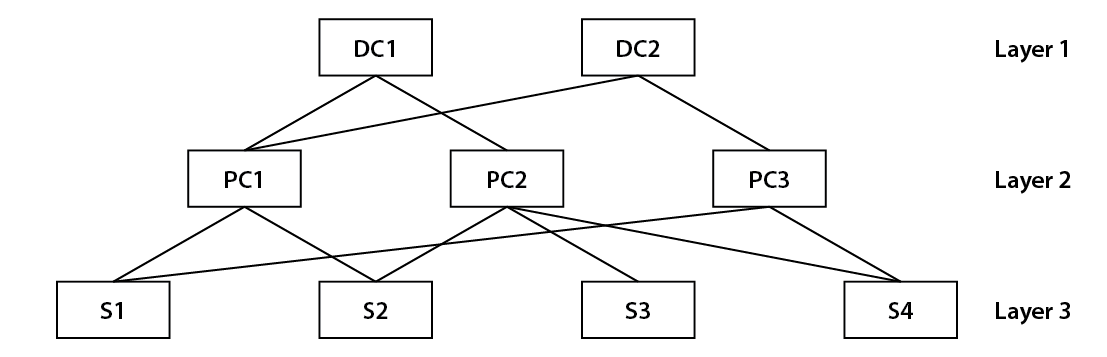
\includegraphics[width = 0.95\linewidth, angle = 0]{figures/Formalisation-04}
\caption{Representation of the belief hierarchy of the agents.}
\label{fig:Formalisation-04}
\end{figure}

Each issue is categorised by three parameters: the actual belief, the preferred state and the preference. The actual belief defines the view of the agent of a certain issue as it is in the environment. They can take values within the interval $[0, 1]$ and where a value of 0.5 means that the agent is satisfied with the issue.

The preferred states shows where the agent would like the issue be in the future. They can also take values within the interval $[0, 1]$.

The preference which is a calculated parameter, defines the urgency that the agent places on the each issues. It is obtained depending on the actual belief, the preferred state and the causal beliefs linked to the issue. The sum of all issue preferences on any single layer of the belief hierarchy have to be equal to 1.

The belief hierarchy structure also contains causal beliefs. These can be seen as causal relations. They represent the understanding of an agent about how a change in one issue will lead to a change in another on a different layer. The causal beliefs can take values within the interval $[-1, 1]$. A negative value means that an issue when growing will affect negatively another issue.

%%%%%% end of the belief system paragraph
%%%%%%%%%%%%%%%% end of the agents subsection


%%%%%%%%%%%%%%%%
\subsection{The actions and interactions}

% preferences calculation
% preferences selection
% agenda selection
% policy instrument selection
% electorate influence

There are a number of actions and interactions that the agents can performed. We will first outline the actions that actors have to make for the system to work. This includes the calculation of the preferences. We will then outline the agenda and policy instrument selection for the entire policy arena. Finally, we outline how we conceptualise that the electorate influence the policy makers.

%%%%%%
\paragraph{Preference calculation - deep core issues}

For the deep core issues, which are at the top of the belief system, the preference is calculated differently than for the policy core and secondary issues. The calculation of the preference for each issue is given by:

\begin{equation}
P_i = \frac{ |G_i - B_i|}{\sum_{j=1}^n |G_j - B_j|}
\end{equation}

where $P$ is the preference, $G$ is the preferred state - or goal, $B$ is the actual belief - or belief, $j$ is defined at the number of principle belief issues and $i$ is the deep core issue.

%%%%%% end of the preference calculation DC issue paragraph

%%%%%%
\paragraph{Preference calculation - policy core and secondary issues}

The preference calculations for the policy core and secondary issues are adapted to include the causal beliefs that link these layers to their directly above layers.

To calculate the preference, the gap between aim and state for the issues is considered along with the impact of the causal relation on the gap of the issue on the above layers. The causal relations are not always helping bridge the gap between the aim and the state of issues on a higher layer. If this is the case, then the causal relations are not considered within the calculation as there effort is counter productive within the mind of the agent. The resulting equation that can be used to calculate the preference for these layers is given by:

\begin{equation}\label{eq:preference2}
P_k = \frac{ |G_k - B_k| + \sum_{j=1}^n |C_j \left( G_j - B_j \right)|}{\sum_{l=1}^p \left[ |G_l - B_l| + \sum_{j=1}^n \left|C_{j,l} \left( G_{j,l} - B_{j,l} \right) \right| \right]}
\end{equation}

The sums only include these terms if $C_j$ and $\left( G_j - B_j \right)$ have the same sign. If it is not the case, these terms are not considered.

Where $p$ is defined at the number of issues on that layer, $k$ characterises the issue being selected for the calculation, $j$ specifies the issues above the layered considered and $C$ represents the causal belief between $k$ and whichever issue on the layer above is considered.

Based on these preferences obtained, the agent will select one issue to advocate. In the agenda setting, the agent will select one policy core issue and for the policy formulation, the agent will select a secondary issue.

%%%%%% end of the preference calculation PC and S issues paragraph

%%%%%%
\paragraph{Agenda selection}

The \emph{agenda} is a 1-tuple given by \texttt{agenda = (issue)} where \texttt{issue} is the policy core issue that is placed on the agenda by all agents.

To constitute the agenda, an issue has to be chosen as a majority issue by all agents in the policy arena. If no majority is obtained on no issue, then the policy formulation cannot happen as now agenda has been selected.

%%%%%% end of the agenda setting paragraph

%%%%%%
\paragraph{Policy instruments}

The policy instruments are measures that can are chosen by the policy makers to impact the environment. To assess the different policy instruments, the different active agents assess the impact of these instruments on the secondary issues in their belief hierarchy. These instruments have an impact on the gap between the states and the aim of each of these issues. The policy instruments can be described as follows:

\begin{enumerate}
\item A \emph{policy instrument} is represented as a 2-tuple \texttt{(ID, impact)} where \texttt{impact} is related to the impact of the policy on a specific issue.

\item There are as many \emph{impacts} of a policy instrument as there are secondary issues. These impacts provide an information to the agents on how much the secondary issue will change if that instrument is implemented.

\end{enumerate}

%%%%%% end of policy instrument paragraph

%%%%%%
\paragraph{Preference calculation - policy instruments}

The policy makers have to select a policy instrument that they will advocate for. This is based on their preferences for which the calculation is detailed below:

\begin{equation}
P_k = \frac{\sum_{p = 0}^{n} | G_{p} - \left( B_{p} (1 + I_{k,p}) \right) |}{\sum_{q = 0}^{m} \sum_{p = 0}^{n} | G_{q} - \left( B_{q} (1 + I_{q,p}) \right) |}
\end{equation}

where $k$ is the policy instrument for which the preference is calculated, $n$ is the number of secondary issues, $m$ is the number of policy instruments, $I$ is the impact of the instrument on a specific secondary issue.

Once all the preferences have been calculated, the agent will select the instrument with the highest preference.

%%%%%% end of the preference calculation policy instrument paragraph

%%%%%%
\paragraph{Policy instrument selection and implementation}

The policy makers are the agents that can selected a policy instrument at the end of the policy formulation step. This is done through a majority vote. If a majority of actors decide on one policy instrument, then that instrument is implemented.

%%%%%% end of policy instrument implementation paragraph

%%%%%%
\paragraph{Electorate passive action on policy makers}

The policy makers are passively influenced by the electorate. Each electorate has a certain affiliation to which policy makers are also related. Each policy makers' issue aim will be influenced by their respective electorate. This happens as a passive effect where the issue aims of the policy makers slowly progress towards the issue aims of the electorate. The equation to calculate the change in the aim of the policy maker is given as follows:

\begin{equation}
G_{k} := G_{k} + \left(G_{El} - G_{k} \right) \cdot C_{i}
\end{equation}

where $El$ stands for electorate of same affiliation of the policy maker, $k$ is a policy maker, $C_i$ is a the constant influence that allows variation in the speed of the change of the goals of the actors.

%%%%%% end of the electorate action paragraph
%%%%%%%%%%%%%%%% end of the actions and interactions subsection
%%%%%%%%%%%%%%%%%%%%%%%%%%%%%%%% end of the formalisation section


%%%%%%%%%%%%%%%%%%%%%%%%%%%%%%%%
\section{Code documentation}

The following is the documentation for the policy process model.

%%%%%%%%%%%%
\subsection{model\_SM.py}

The \texttt{model\_SM.py} is the main file fo the policy emergence model. This is where the policy process is coded and stepped through. The different functions of this files are outlined below:

\begin{itemize}
\item \texttt{get\_agents\_attributes()}

This function is used as part of the datacollector function. This function is used to output the key attributed of the policy emergence model agents. Note that a deepcopy function is used for to avoid data rewriting over itself.

\item \texttt{get\_electorate\_attributes()}

This function is similar to the previous one but for the electorate attributes.

\item \texttt{get\_problem\_policy\_chosen()}

This function is also used as part of the datacollector function. This function records the agenda selected and the policy implemented by the agents.

\item \texttt{step()}

The step function is the main core of policy emergence model. It consists of a set of steps. These are the initialisation, the agenda setting, the policy formulation and the data collection. For the initialisation, this includes the communication of the beliefs from the environment and the impact of the policy instruments to the agents.

\item \texttt{module\_interface\_input()}

The module interface function is used to inform the active agents of what has happened in the environment. This includes taking the indicators and feeding them to the truth agent. Taking the truth agents issue tree and informing all active agents. Finally, it includes informing the active agents about the policy instruments' impact that are recalculated for every step of the policy emergence model.

\item \texttt{agenda\_setting()}

In the agenda setting step, the active agents first select their policy core issue of preference and then select the agenda. Then we check for all preferences for all agents and see whether there is a majority of one policy core issue. If that is the case, then the policy formulation can happen.
		
\item \texttt{policy\_formulation()}

In the policy formulation step, the policy maker agents first select their policy core issue of preference and then they select the policy that is to be implemented if there is a majority of them.

\item \texttt{preference\_update()}

This function is used to call the preference update functions of the issues of the active agents.

\item \texttt{preference\_update\_DC()}

This function is used to update the preferences of the deep core issues of agents in their respective issue trees.

\item \texttt{preference\_update\_PC()}

This function is used to update the preferences of the policy core issues of agents in their respective issue trees.
		
\item \texttt{preference\_update\_S()}

This function is used to update the preferences of secondary issues the agents in their respective issue trees.

\item \texttt{electorate\_influence()}

This function calls the influence actions in the electorate agent class.

\end{itemize}

%%%%%%%%%%%% end of model\_SM.py

%%%%%%%%%%%%
\subsection{model\_SM\_agents.py}

\begin{itemize}
\item \texttt{ActiveAgent} class:

The active agent class contains the policy makers and the policy entrepreneurs. These are agents that have a say in the agenda setting and the policy formulation.

	\begin{itemize}
	\item \texttt{selection\_PC()}
	
	This function is used to select the preferred policy core issue for the active agents based on all their preferences for the policy core issues.
	
	\item \texttt{selection\_S()}
	
	This function is used to select the preferred secondary issue. First, only the secondary issues that are related, through a causal relation, to the policy core issue on the agenda are placed into an array. Then, the one with the highest preference is selected. It is then used as the issue that the agent will advocate for later on.
	\item \texttt{selection\_PI()}
	
	This function is used to select the preferred policy instrument from the policy family on the agenda. First the preferences are calculated. Then the policy family preferred is selected as the policy family with the lowest preference (this means the smallest gap after the introduction of the policy family likelihood).

	\end{itemize}

\item \texttt{ElectorateAgent} class:

This is the electorate agent class. These agents are only used to influence the policy makers. They cannot be influenced by agents within the system.

	\begin{itemize}
	\item \texttt{electorate\_influence()}
	
	This function is used to perform the electorate influence on the policy makers.
	\end{itemize}
	
\item \texttt{TruthAgent} class:

This is the truth agent class. It is used to transfer the indicators into beliefs for the active agents.

\end{itemize}

%%%%%%%%%%%% end of model\_SM\_agents.py


%%%%%%%%%%%%
\subsection{model\_SM\_agents\_initialisation.py}

\begin{itemize}
\item \texttt{issuetree\_creation()}

This function is used to create a skeleton issue tree. This stores all of the issues of the agents.

\item \texttt{policytree\_creation()}

This function is used to create a skeleton policy tree. This stores all of the policy instruments of the agents.

\item \texttt{init\_active\_agents()}

This function creates all of the active agents that are specified within the inputs of the model.

\item \texttt{init\_electorate\_agents()}

This function creates the electorate passive agents. The electorate 

\item \texttt{init\_truth\_agent()}

This function is used to create the truth agent. It has a limited set of attributes and a different structure for its policy tree (it does not need any causal relations).

\end{itemize}


%%%%%%%%%%%% end of model\_SM\_agents\_initialisation.py

%%%%%%%%%%%%
\subsection{model\_SM\_policyImpact.py}

This script is used to calculate the impact of the policy instruments. It is done by simulating a separate instance of the model with a specific policy instrument and by recording the outcome. Such simulation are done using parallel processes. Two functions are considered within this script:

\begin{itemize}
\item \texttt{model\_simulation()}

This function is used to run the independent simulations of the model. It takes in the inputs from the model and outputs the indicators as a result from the simulation.

\item \texttt{policy\_impact\_evaluation()}

This function is used to estimate the impact of the policy instruments on the policy context. This is done by separately simulating every policy instruments and comparing the results with the initial states of the policy context. This is what is then used to inform the agents on the impact of the policies.

\end{itemize}

%%%%%%%%%%%% end of model\_SM\_policyImpact.py
%%%%%%%%%%%%%%%%%%%%%%%%%%%%%%%% end of the code documentation section


%%%%%%%%%%%%%%%%
\appendix
%%%%%%%%%%%%%%%% end of the appendix


%%%%%%%%%%%%%%%%
\bibliographystyle{apalike} 
\bibliography{references}
%%%%%%%%%%%%%%%% end of the bibliography

\end{document}
